\makeatletter\let\ifGm@compatii\relax\makeatother
\documentclass{beamer}
\usepackage{amsfonts}
\usepackage{amsmath}
\usepackage{graphicx}
\usepackage{amssymb}
\usepackage{bm}
\usepackage{movie15}
\usepackage{color}
\usepackage{fancybox}
\DeclareRobustCommand{\orderof}{\ensuremath{\mathcal{O}}}

\mode<presentation>
{
   \usetheme{Boadilla}
}



\title[Physical properties of LiF-ThF$_4$]
{
Predictions of physical properties of LiF-ThF$_4$ \\ from molecular dynamics simulations 
}
\author[M. Levesque]{
  Maximilien Levesque, Paul Madden, Mathieu Salanne, \\ Christian Simon, Aimen Gheribi \& Patrice Chartrand}
\institute[UPMC]{
  Universit\'e Pierre et Marie Curie -- Paris -- France  \\
  University of Oxford -- UK \\
  Polytechnique Montreal -- Canada
} 
\date[June 28, 2013]{\alert{EVOL meeting - June 28, 2013}}

\begin{document}

\makeatletter
  \@ifundefined{inserttotalframenumbernew}{
    \gdef\inserttotalframenumbernew{1}
  }{}
  \gdef\inserttotalframenumber{\inserttotalframenumbernew}
\makeatother

\begin{frame}
 \titlepage
\end{frame}




\begin{frame}
  \frametitle{Outline}
  \tableofcontents
\end{frame}

\section{MD simulations}

\begin{frame}
   \frametitle{Simulation method: molecular dynamics}
   \begin{columns}
      \begin{column}{6cm}
         \begin{itemize}
            \item[$\bullet$] Newton's equation of motion solved at each time step:\\
            \begin{equation}m^i\ddot{\vec{r}}^i=\sum_{j\ne i}\vec{F}^{j\rightarrow i}=-\frac{\partial V}{\partial \vec{r}^i}\nonumber\end{equation}\\
            where $V$ is the \alert{interaction potential}
  
            \item[$\bullet$] Trajectory of particles over a few nanoseconds
            \item[$\bullet$] Determination of \alert{structural}, \alert{thermodynamic} and \alert{transport} properties
         \end{itemize}
      \end{column}
      \begin{column}{6cm}
         \begin{figure}
            \includemovie[poster,text={Loading movie}]{6cm}{6cm}{sio2na2o.mpg}
         \end{figure}
         \vspace{-0.5cm}
         \begin{center}
            {\small \it Simulation cell for SiO$_2$-Na$_2$O}
         \end{center}
      \end{column}
   \end{columns}
\end{frame}

\begin{frame}
   \frametitle{Testing the potentials: LiF-ThF$_4$}

   \begin{figure}
   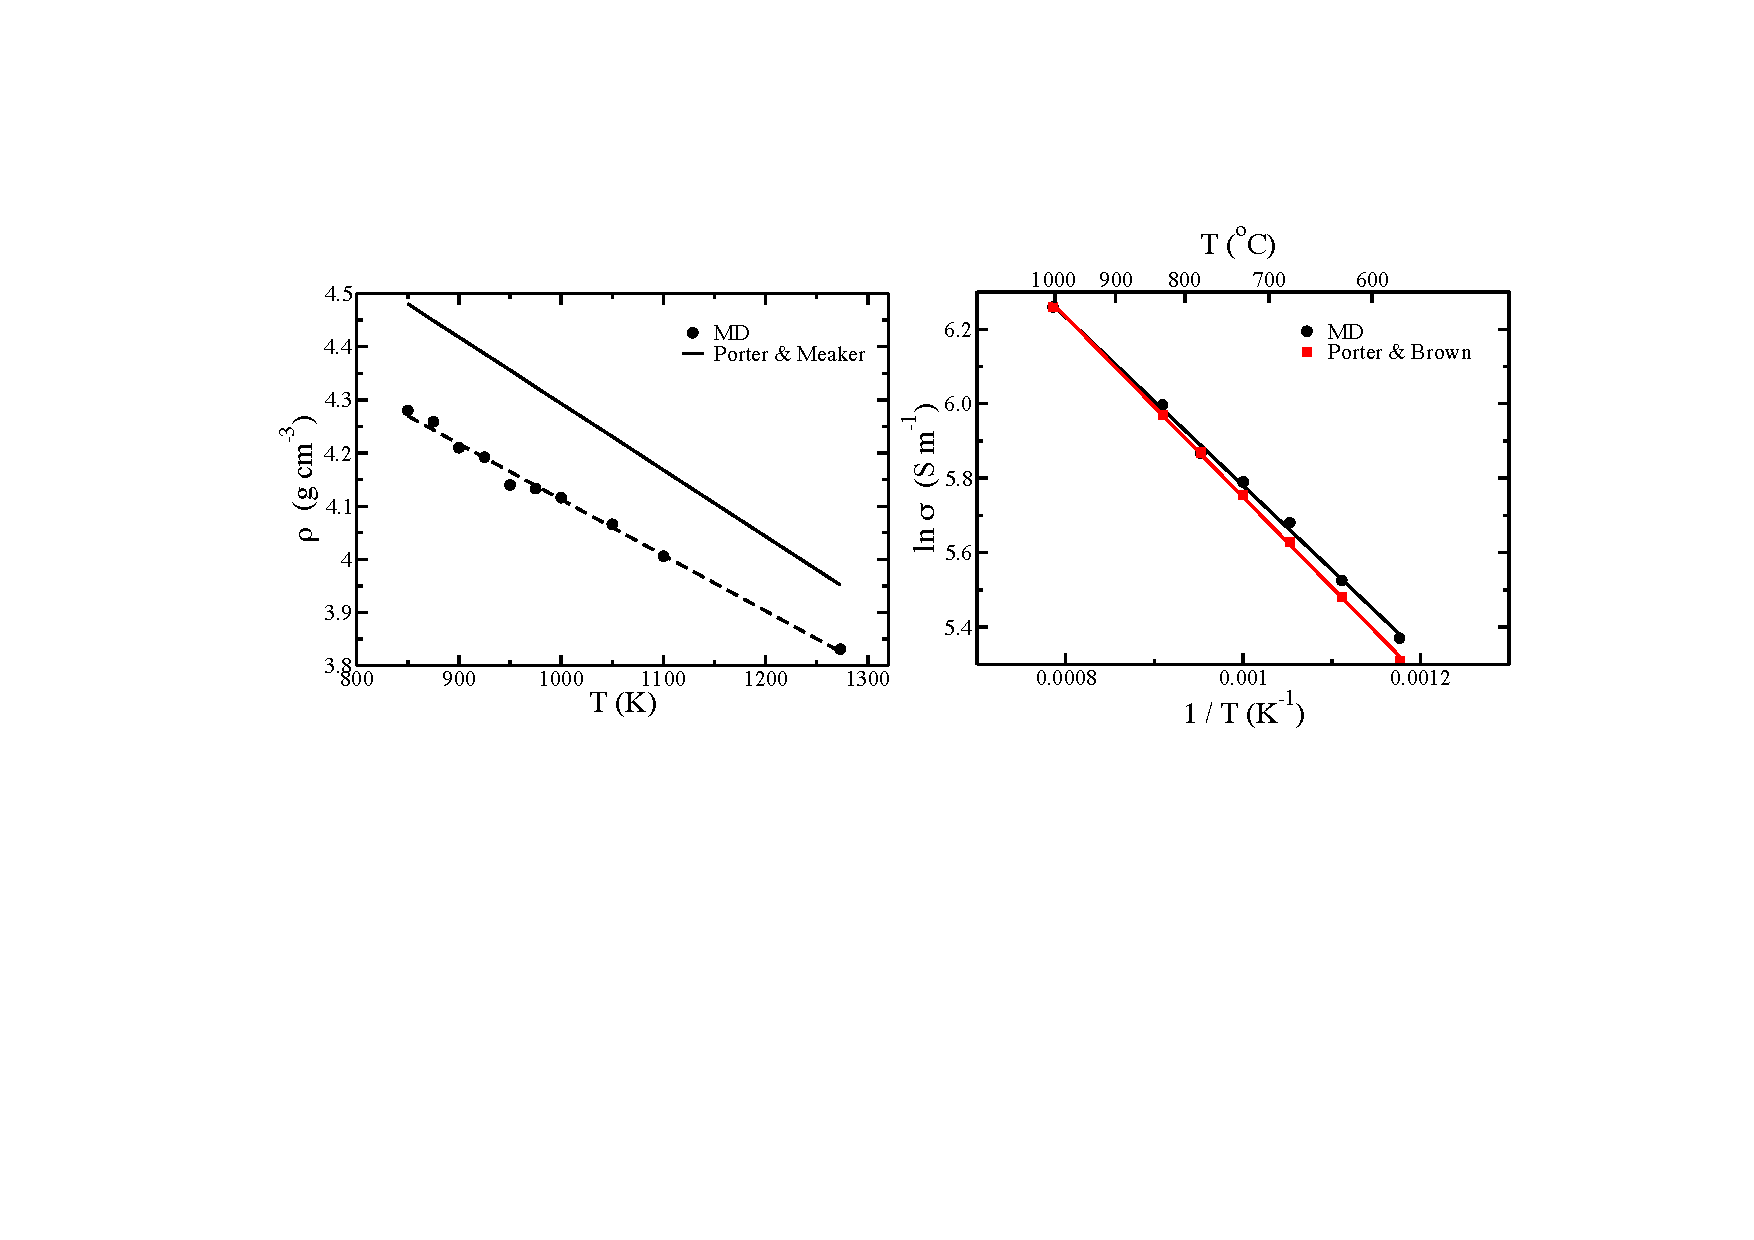
\includegraphics[width=\textwidth]{dewan-valid}
   \end{figure}

   \begin{columns}
      \begin{column}{6cm}
        \begin{itemize}
           \item[$\bullet$] Underestimation of \\ the density by $\approx$4~\%
        \end{itemize}
      \end{column}
      \begin{column}{6cm}
        \begin{itemize}
           \item[$\bullet$] Excellent accuracy \\ for the conductivity
        \end{itemize}
      \end{column}
   \end{columns}
\vspace{0.5cm}

\begin{center}
$\rightarrow$ Possible to predict all the other properties!
\end{center}

   \scriptsize{Dewan, Simon, Madden, Hobbs \& Salanne, {\it J. Nucl. Mater.}, 434, 322 (2013)}
\end{frame}

%~ 
\begin{frame}
   \frametitle{Testing the potentials: LiF-YF$_3$}


   \begin{columns}
      \begin{column}{6cm}
         \begin{figure}
   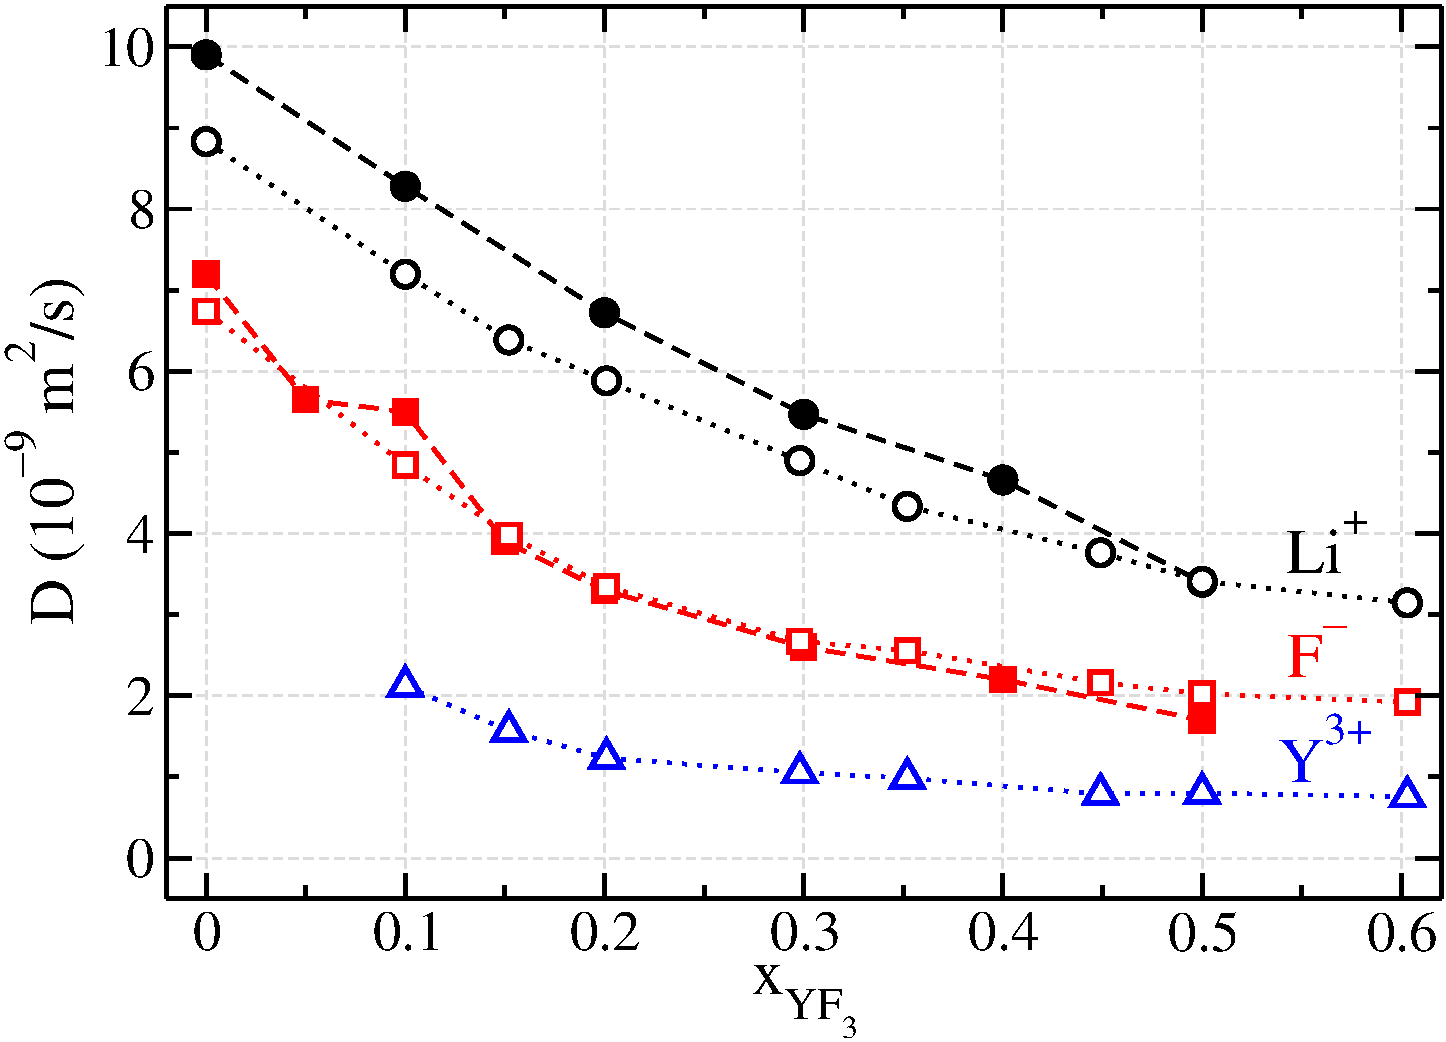
\includegraphics[width=\textwidth]{LiFYF3diffusion}
   \end{figure}

        \begin{itemize}
           \item[$\bullet$] Good approximation of \\ macroscopic transport properties
        \end{itemize}
      \end{column}
      \begin{column}{6cm}
               \begin{figure}
   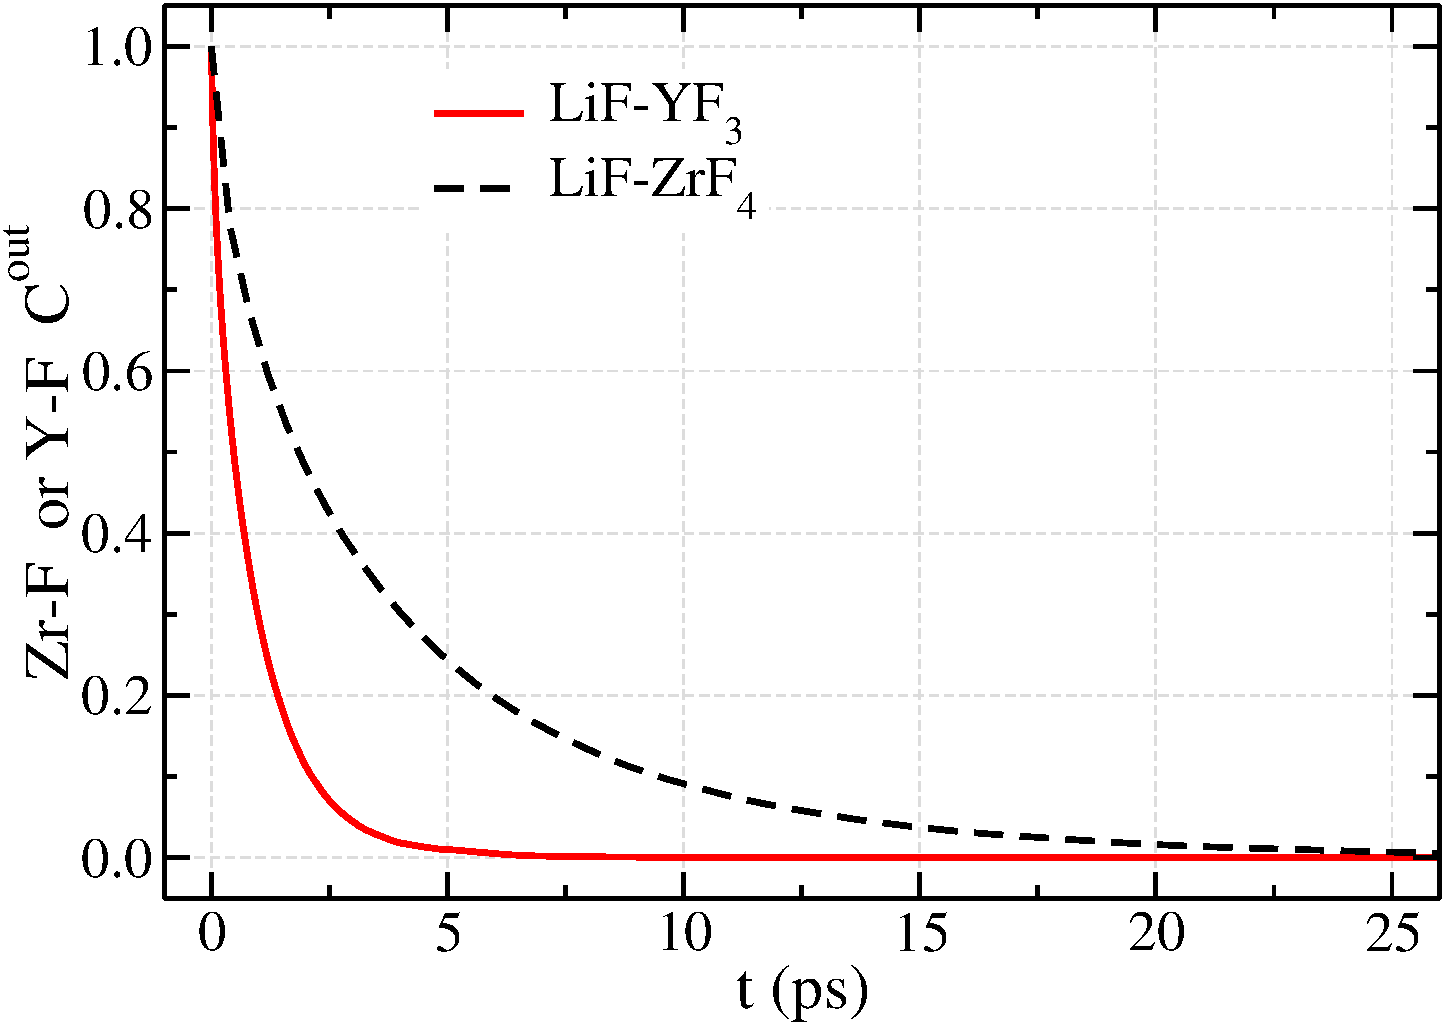
\includegraphics[width=\textwidth]{LiFYF3cage}
   \end{figure}

        \begin{itemize}
           \item[$\bullet$] Access to molecular correlation functions and more!
        \end{itemize}
      \end{column}
   \end{columns}
\begin{center}
$\rightarrow$ Prediction of macroscopic properties\\
$\rightarrow$ Understanding of molecular origin!
\end{center}

   \scriptsize{Levesque {\it et al.}, {\it J. Chem. Phys.} {\bf 138}, 184503 (2013)}
\end{frame}
%~ 






\AtBeginSection[]
{
  \begin{frame}<beamer>
    \frametitle{Outline}
    \tableofcontents[current,currentsection]
  \end{frame}
}


\section{LiF-ThF$_4$ mixtures}

\begin{frame}
   \frametitle{Density of LiF-ThF$_4$ mixtures}
   \begin{figure}
   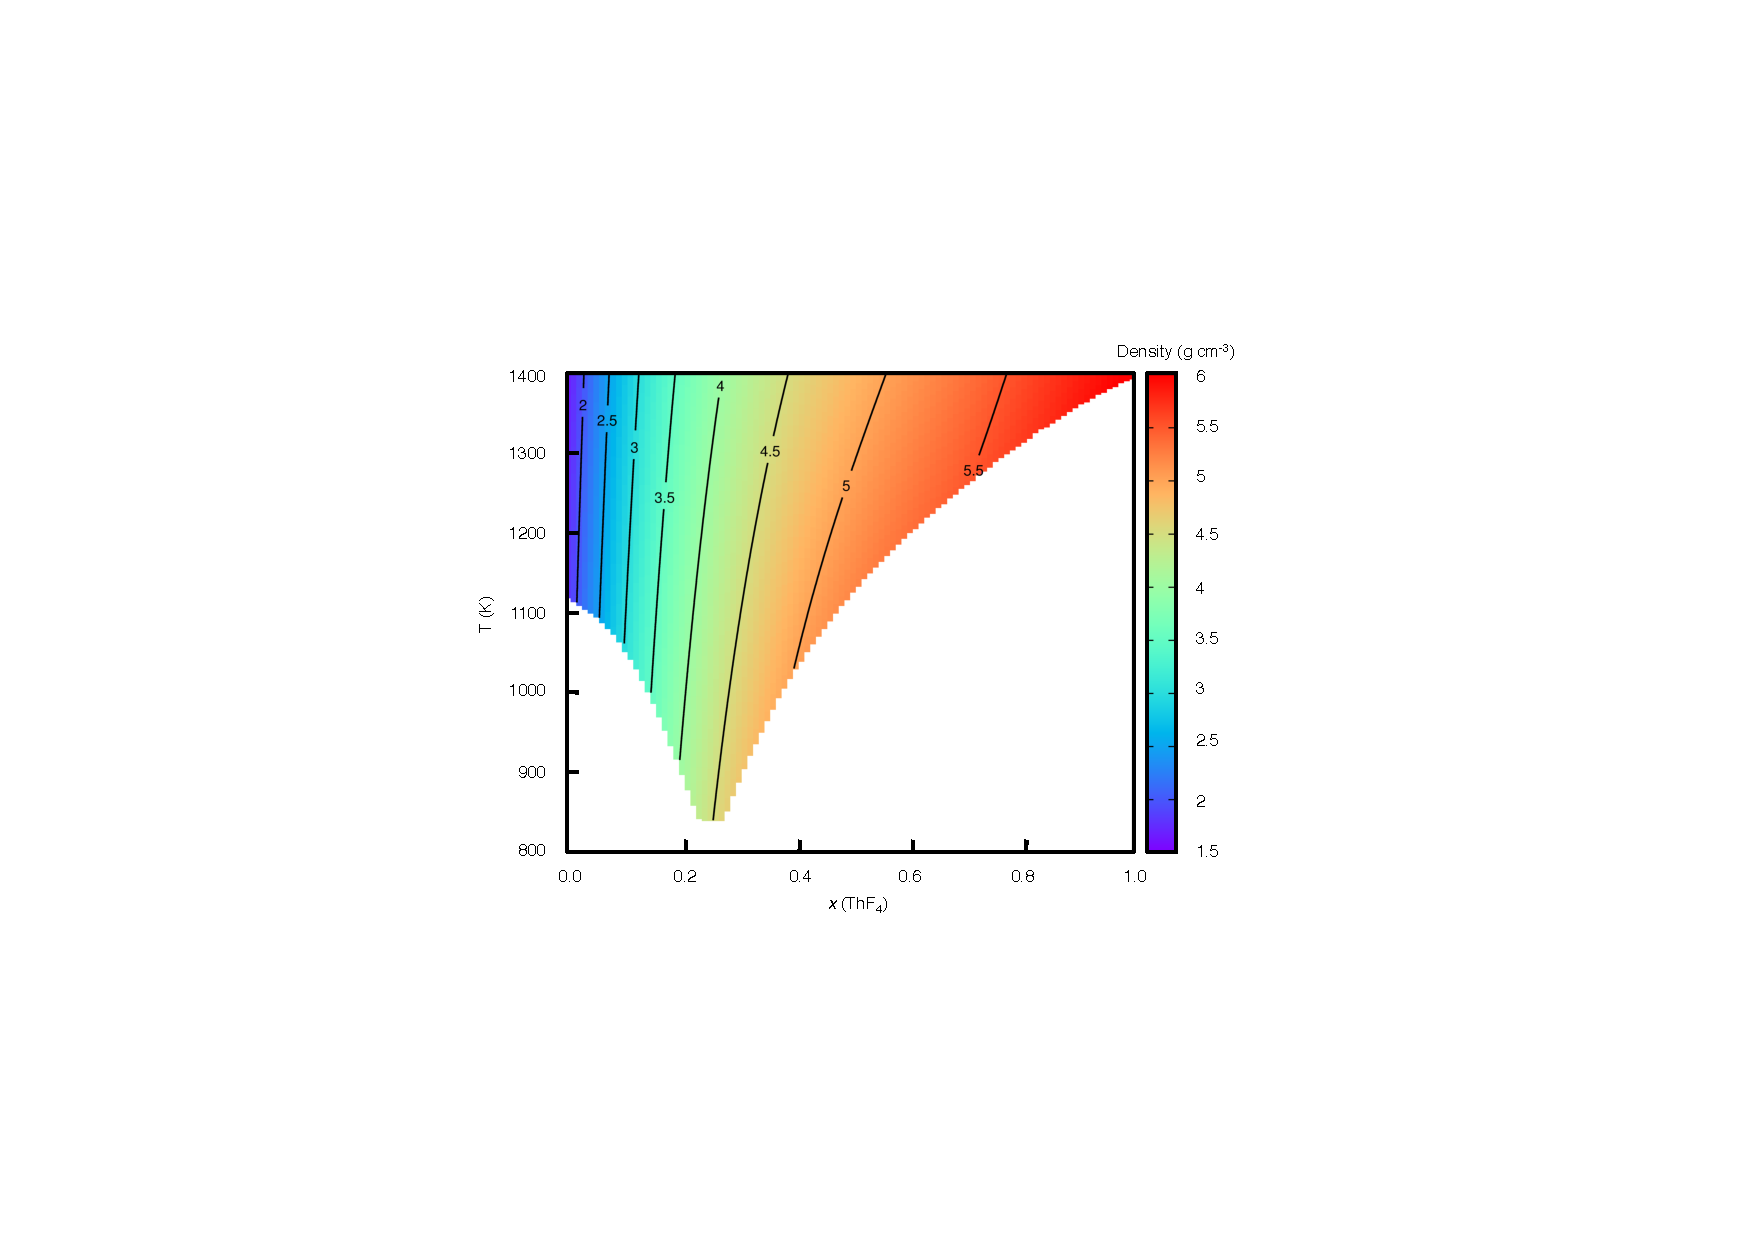
\includegraphics[width=.6\textwidth]{density}
   \end{figure}

   Calculations made for 40 different ($x_{\rm ThF_4}$, T) couples\\ and polynomial fit of the data
   
\end{frame}

\begin{frame}
   \frametitle{Viscosity of LiF-ThF$_4$ mixtures}
   \begin{figure}
   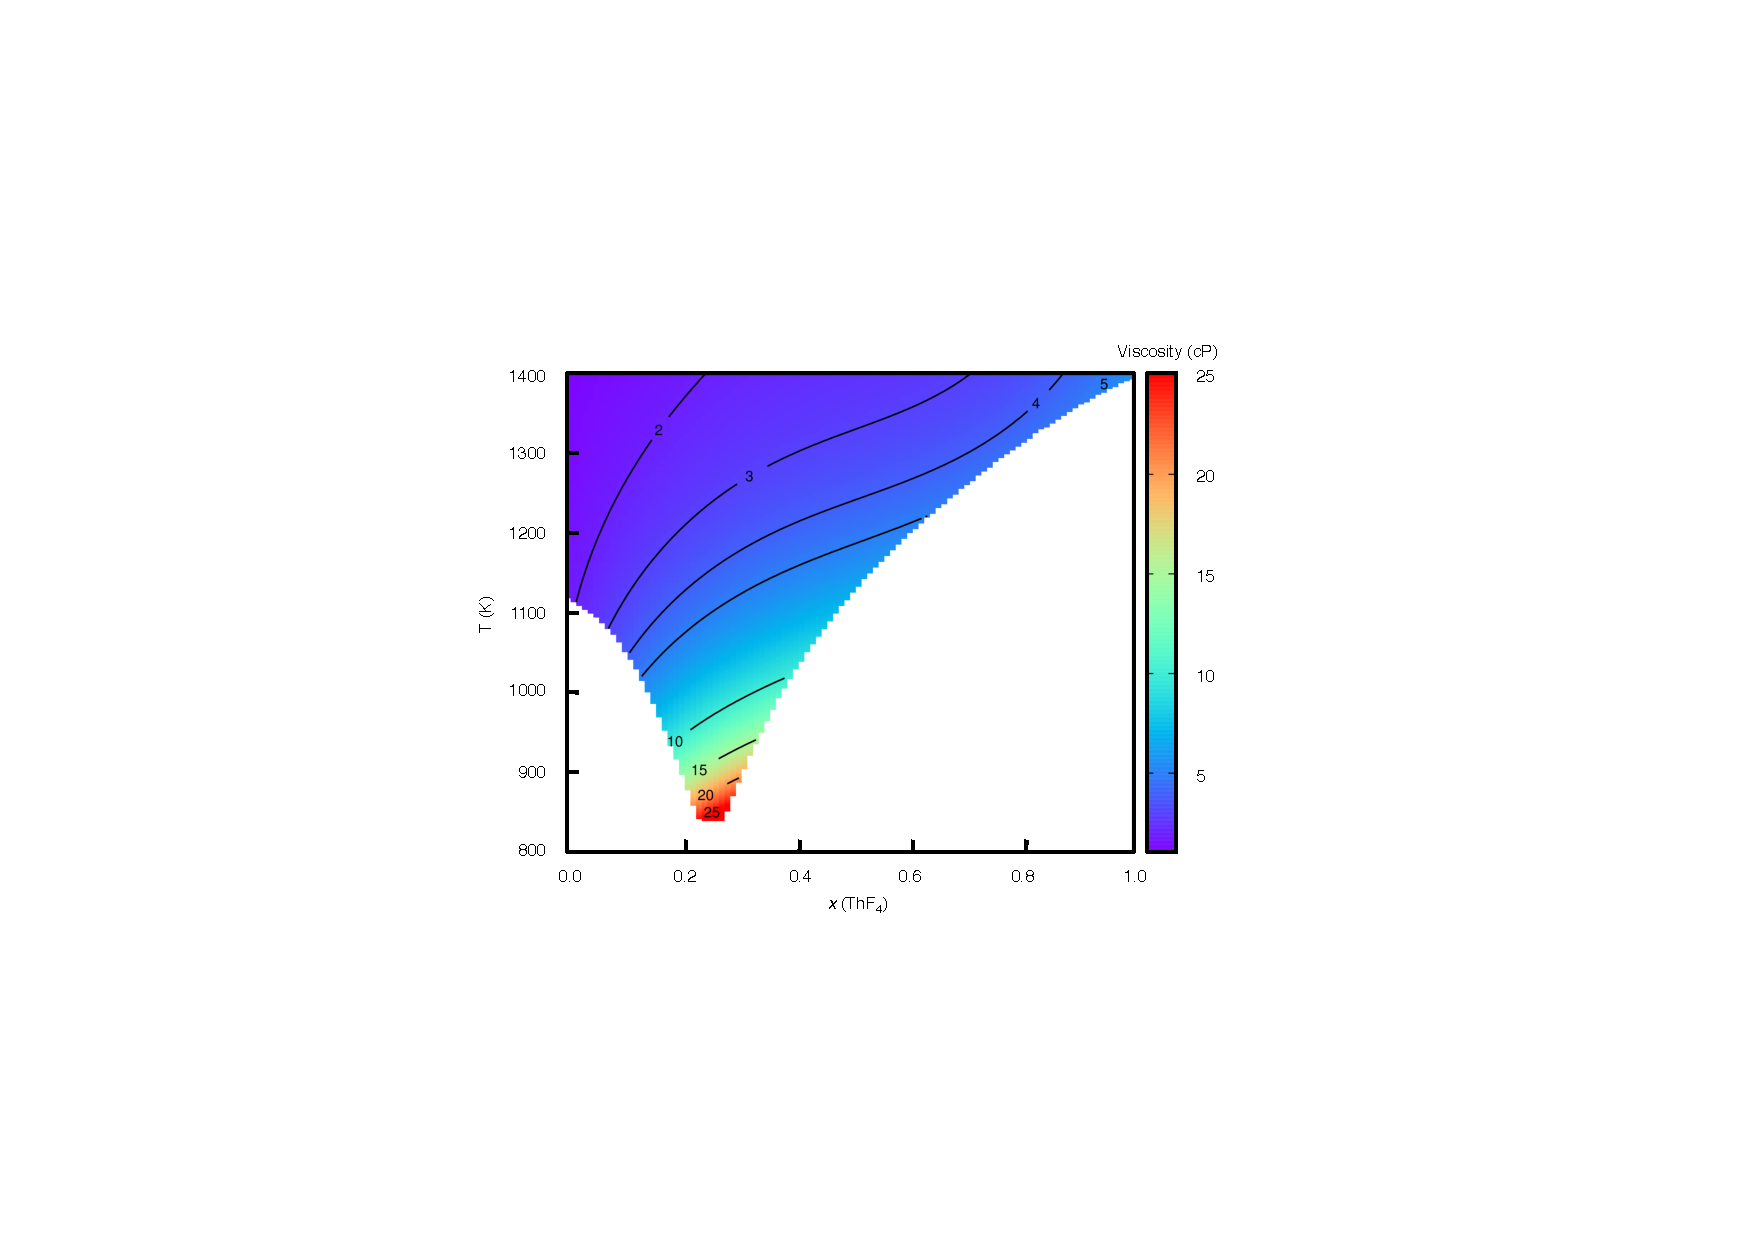
\includegraphics[width=.6\textwidth]{viscosity}
   \end{figure}

   Calculations made for 30 different ($x_{\rm ThF_4}$, T) couples\\ and polynomial fit of the data
   
\end{frame}

\begin{frame}
   \frametitle{Figures of merit}
         \[
         FOM=\frac{\eta^x}{\beta^y\rho^z C_p^t \lambda_T^u}
         \]
      \begin{itemize}
      \item[$\bullet$] $C_p$ heat capacity
      \item[$\bullet$] $\rho$ density
      \item[$\bullet$] $\eta$ viscosity
      \item[$\bullet$]  $\beta$ thermal expansion
      \item[$\bullet$] $\lambda_T$ thermal conductivity
   \end{itemize}

\vspace{1cm}
{\scriptsize  C. Bonilla, {\it Nuclear Engineering Handbook}, 9-90 (1958)}
\end{frame}

\begin{frame}
   \frametitle{Forced convection, turbulent r\'egime}
   \begin{figure}
   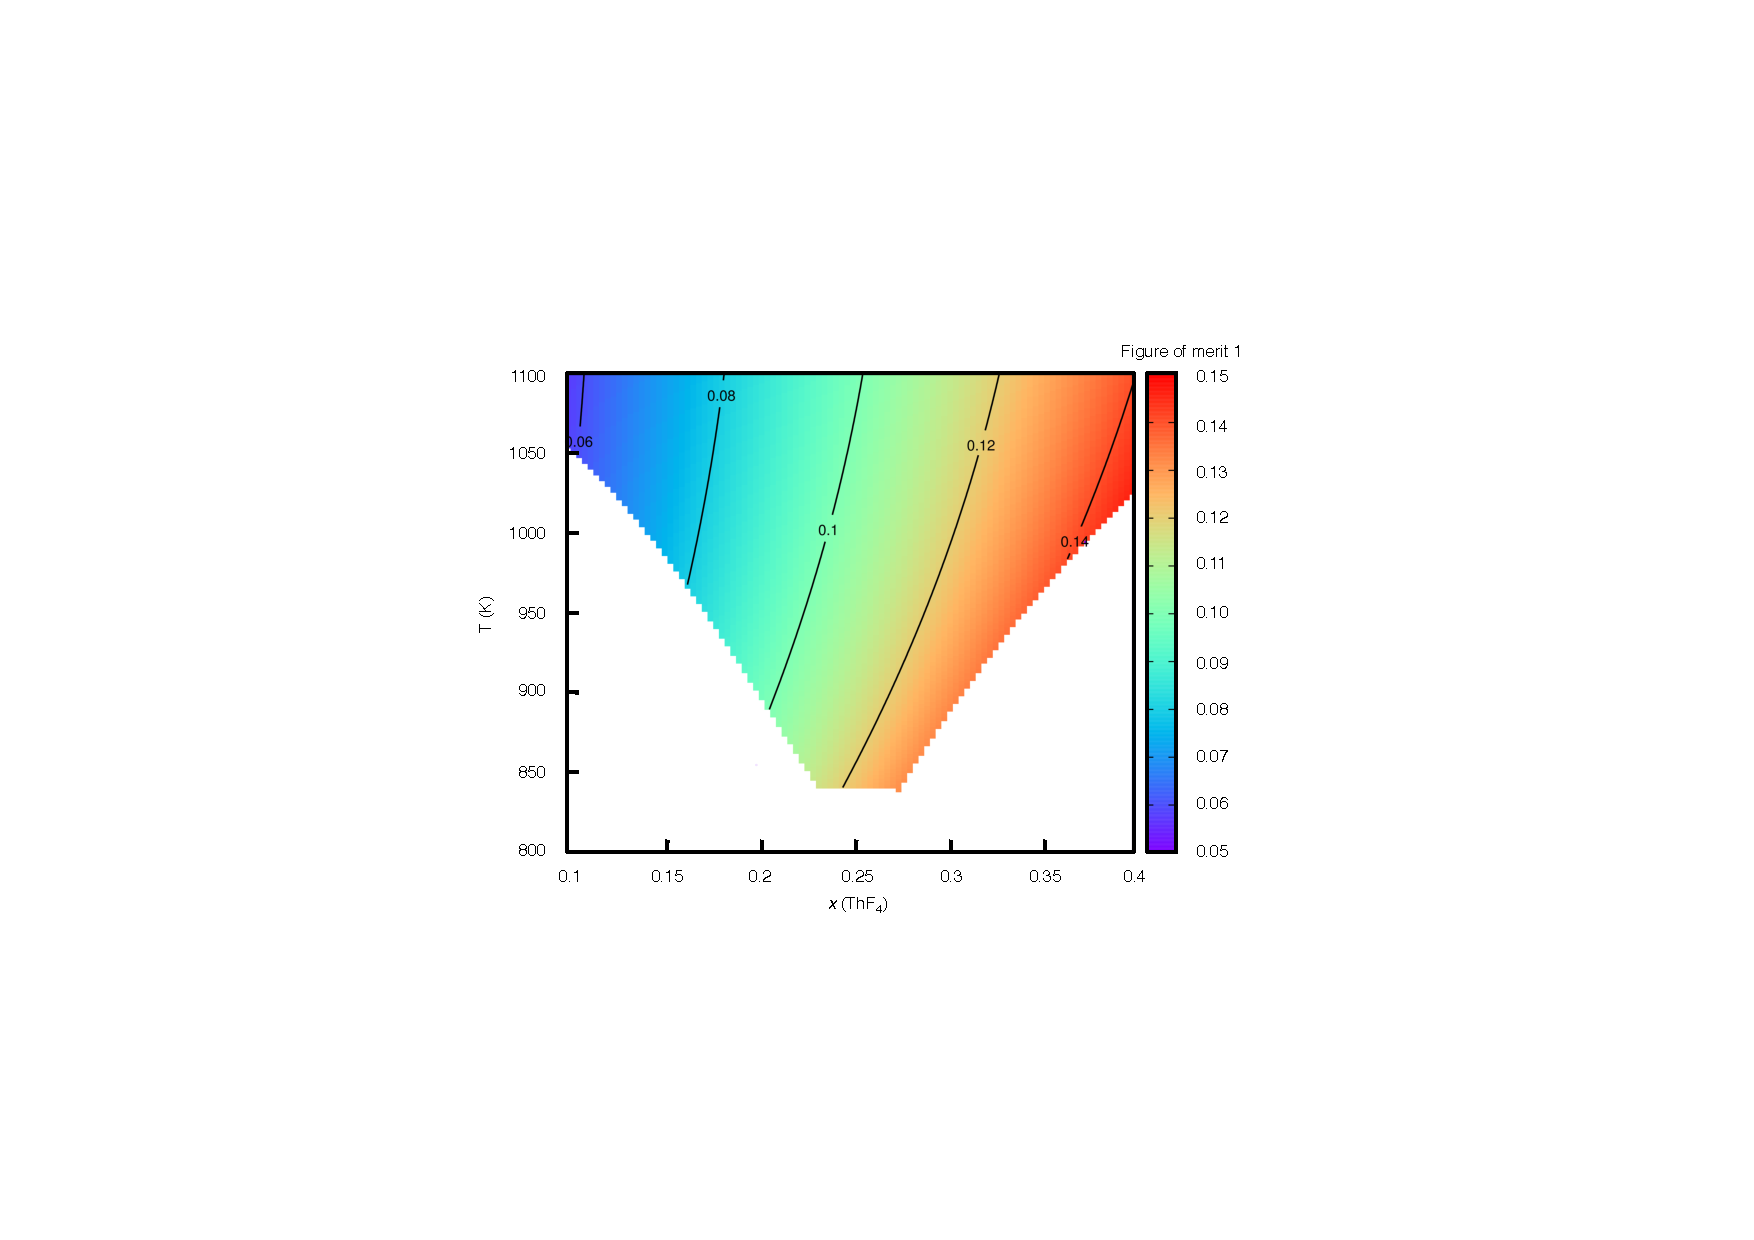
\includegraphics[width=.6\textwidth]{merit1}
   \end{figure}

  Other salts at 873~K:
    \begin{columns}
      \begin{column}{6cm}
        \begin{itemize}
           \item[$\bullet$] FLiNaK: 0.063
        \end{itemize}
      \end{column}
      \begin{column}{6cm}
        \begin{itemize}
           \item[$\bullet$] NaF-ZrF$_4$ eutectic: 0.126
        \end{itemize}
      \end{column}
   \end{columns}
   
\end{frame}

\begin{frame}
   \frametitle{Natural convection, turbulent r\'egime}
   \begin{figure}
   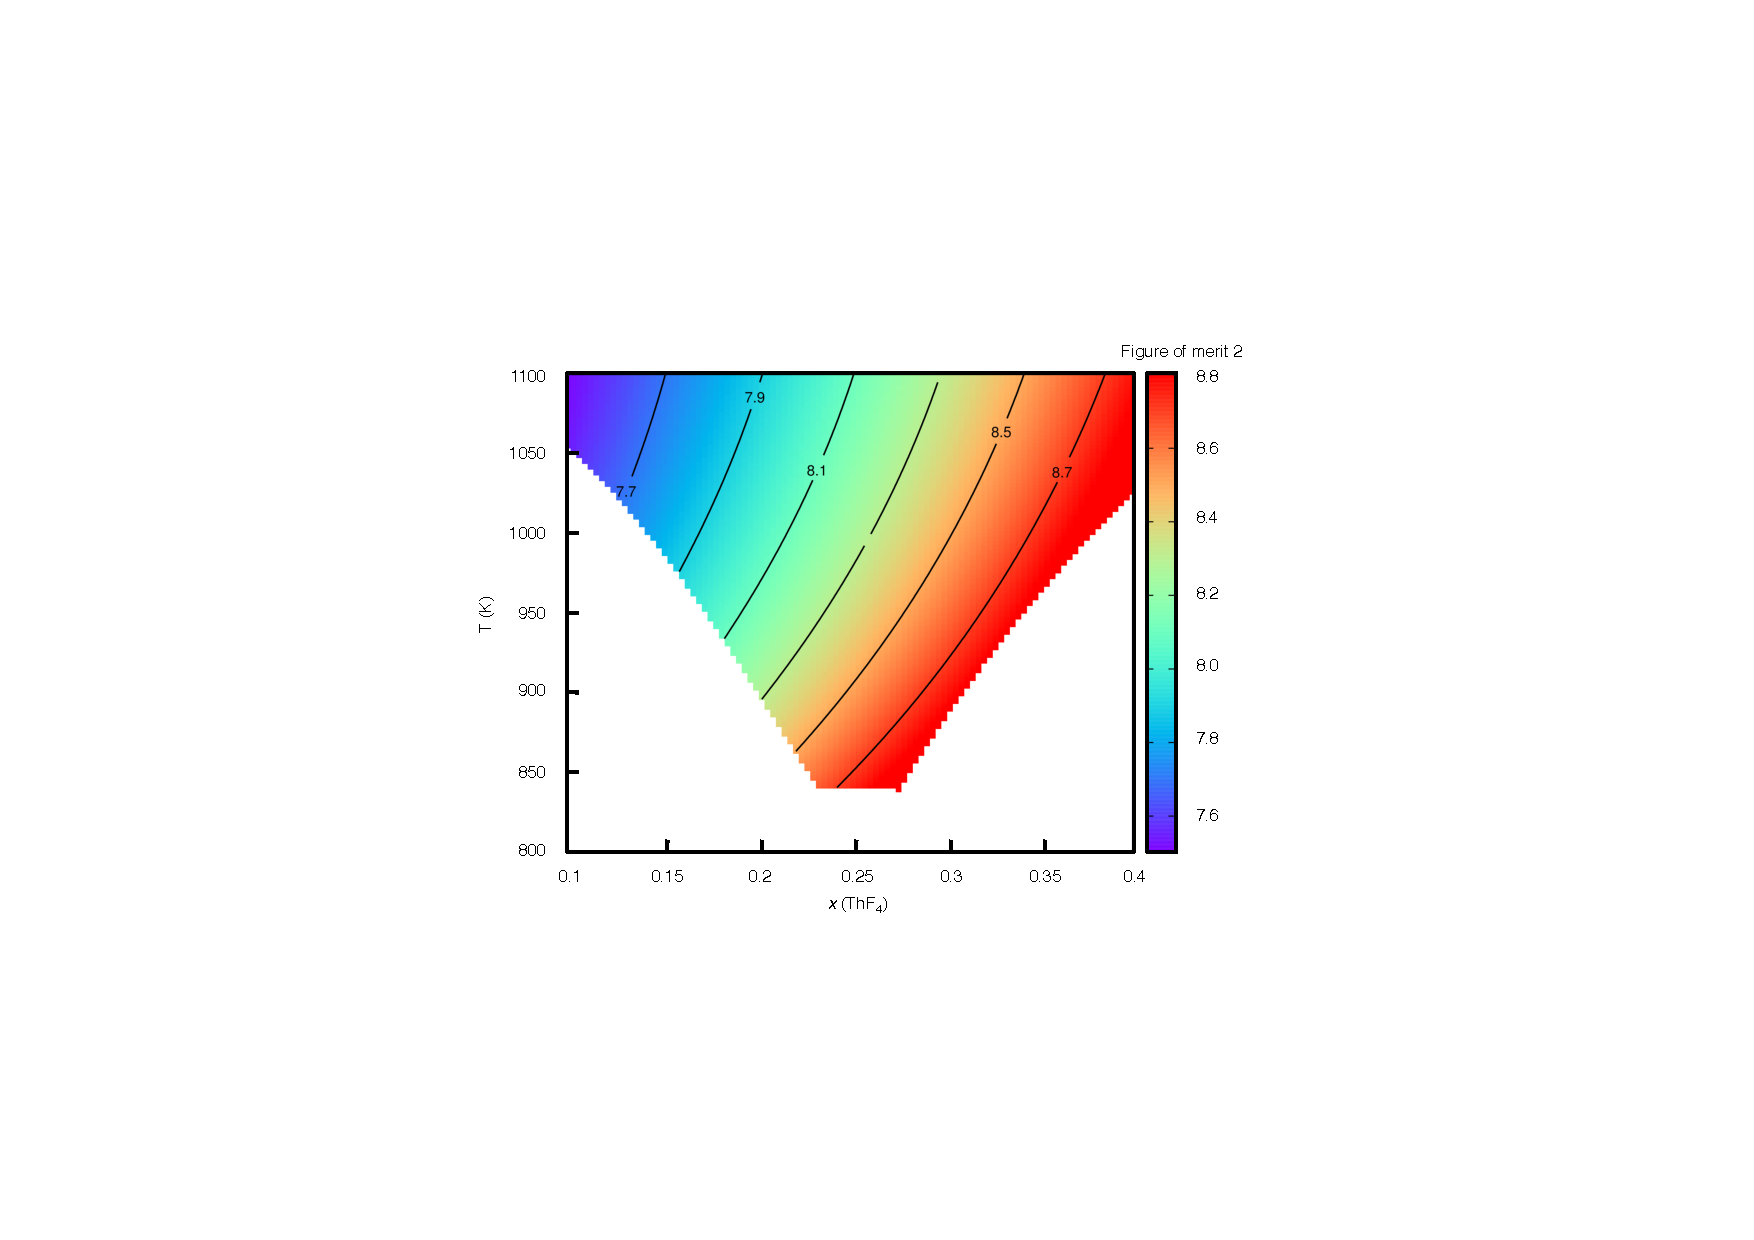
\includegraphics[width=.6\textwidth]{merit2}
   \end{figure}

  Other salts at 873~K:
    \begin{columns}
      \begin{column}{6cm}
        \begin{itemize}
           \item[$\bullet$] FLiNaK: 8.01 
        \end{itemize}
      \end{column}
      \begin{column}{6cm}
        \begin{itemize}
           \item[$\bullet$] NaF-ZrF$_4$ eutectic: 8.98
        \end{itemize}
      \end{column}
   \end{columns}
   
\end{frame}

\begin{frame}
   \frametitle{Natural convection, laminar r\'egime}
   \begin{figure}
   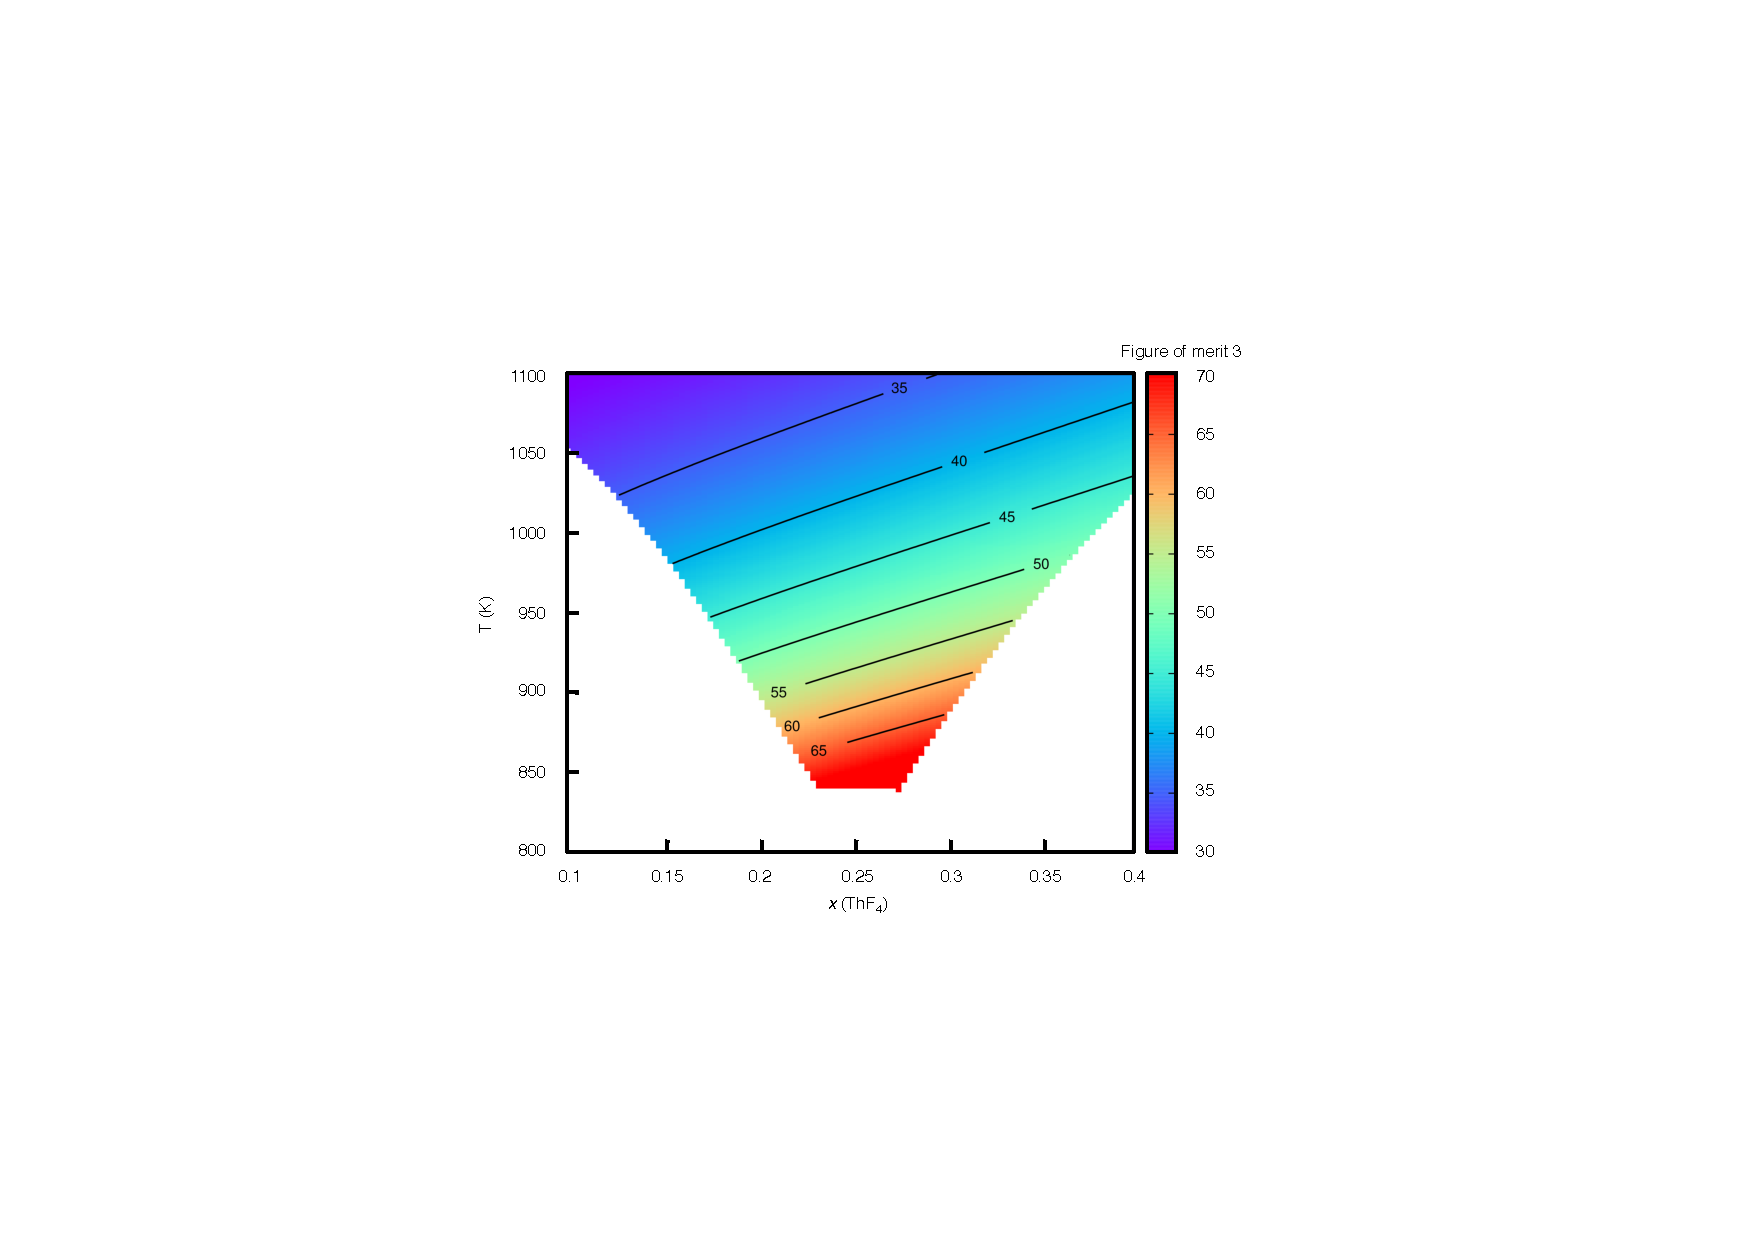
\includegraphics[width=.6\textwidth]{merit3}
   \end{figure}

  Other salts at 873~K:
    \begin{columns}
      \begin{column}{6cm}
        \begin{itemize}
           \item[$\bullet$] FLiNaK: 31.45
        \end{itemize}
      \end{column}
      \begin{column}{6cm}
        \begin{itemize}
           \item[$\bullet$] NaF-ZrF$_4$ eutectic: 41.74
        \end{itemize}
      \end{column}
   \end{columns}
   
\end{frame}
%~ 
%~ 
%~ 
%~ 
%~ 
%~ 
%~ 
%~ 
%~ 
%~ 
\section{Activity coefficients}
%~ 
%~ 
%~ 
%~ 
\begin{frame}{Objective}
    \begin{itemize}
        \item Predict solubilities when experimentally difficult to measure
        \item $\Rightarrow$ e.g. Pu in LiF-ThF$_4$ (what quantity of Pu can be dissolved).
        \item Saddly, it is also difficult from a theoretical and numerical point of view.
        \begin{itemize}
            \item clear definition of the chemical potential(s)
            \item and of the reference state?
            \item Necessity for workarounds?
            \item Specific needs $\Rightarrow$ specific codes! (on the basis of Paul's codes)
        \end{itemize}
    \end{itemize}
    \scriptsize{Salanne, Simon, Turq \& Madden, JPCB 112, 1177 (2008)}
\end{frame}
%~ 
%~ 
%~ 
%~ 
\begin{frame}
    \frametitle{We measure activity coefficients, not solubilities}{}
    \begin{itemize}
        \item Equilibrium:
            \begin{center}
                A(dissolved in S) + B(solid) = A(solid) + B(dissolved in S)\\
                A = e.g. YF$_3$, B = e.g. PuF$_3$
            \end{center}
        \item Associated reversible work (Gibbs free energy):
            \begin{equation}
                \beta \Delta G_\text{tot} = \ln\left(\frac{\gamma_B^S}{\gamma_A^S}\right) +\beta \Delta \mu ^0 \nonumber
            \end{equation}
            $\gamma_A^S$ and $\gamma_B^S$: activity coefficients of A and B in salt S.
        \item Link with solubility:
            \begin{equation}
                \frac{\gamma_B^S}{\gamma_A^S} \approx \frac{s_A^S}{s_B^S}   \nonumber
            \end{equation}
        \item $\Delta\mu^0$ unknown $\rightarrow$ use two salts
    \end{itemize}
    \scriptsize{Salanne, Simon, Turq \& Madden, J. Phys. Chem. B \textbf{112}, 1177 (2008)}
\end{frame}
%~ 
%~ 
%~ 
%~ 
\begin{frame}
    \frametitle{Activity coefficients to predict solubilities}
    \begin{itemize}
        \item Two equilibriums:\\
            A(dissolved in S) + B(solid) = A(solid) + B(dissolved in S)\\
            A(dissolved in S$^\prime$) + B(solid) = A(solid) + B(dissolved in S$^\prime$)
        \item
            \begin{eqnarray}
                \Delta G_\text{tot} - \Delta G_\text{tot}^\prime &=& \beta^{-1}\ln\left(\frac{\gamma_B^S}{\gamma_A^S}\right) + \Delta \mu ^0  - \beta^{-1}\ln\left(\frac{\gamma_B^{S^\prime}}{\gamma_A^{S^\prime}}\right) - \Delta \mu ^0 \\ \nonumber
                &=& \beta^{-1}\ln\left(\frac{\gamma_A^{S^{\prime}}\cdot\gamma_B^S}{\gamma_A^S\cdot\gamma_B^{S^\prime}}\right) \\ \nonumber
                &=& \Delta G_{\text{transmut},A\rightarrow B\text{ in S}} - \Delta G_{\text{transmut},A\rightarrow B\text{ in S}^{\prime}} \\ \nonumber
                &\approx & \beta^{-1}\ln\left(\frac{s_A^S\cdot s_B^{S^\prime}}{s_A^{S^{\prime}}\cdot s_B^S}\right)   \nonumber
            \end{eqnarray}
        \item From Ward et al., ORNL (1959) $\rightarrow$ solubility of YF3 and LaF3 in NaF-ZrF$_4$ and NaF-BeF$_2$
    \end{itemize}
\end{frame}
%~ 
%~ 
%~ 
%~ 
\begin{frame}
    \frametitle{How we calculate activity coefficients, or $\Delta G_{\text{transmut},A\rightarrow B\text{ in S}}$}
    \begin{enumerate}
        \item Slowly transmute YF$_3$ into LaF$_3$ in NaF-ZrF$_4$ at given c,T\\ during molecular dynamic simulation
        \item Store average change in internal energy due to transmutation
        %~ figure des transmutation, explication dudl/dl, figure integration pour exemple
            \begin{figure}
                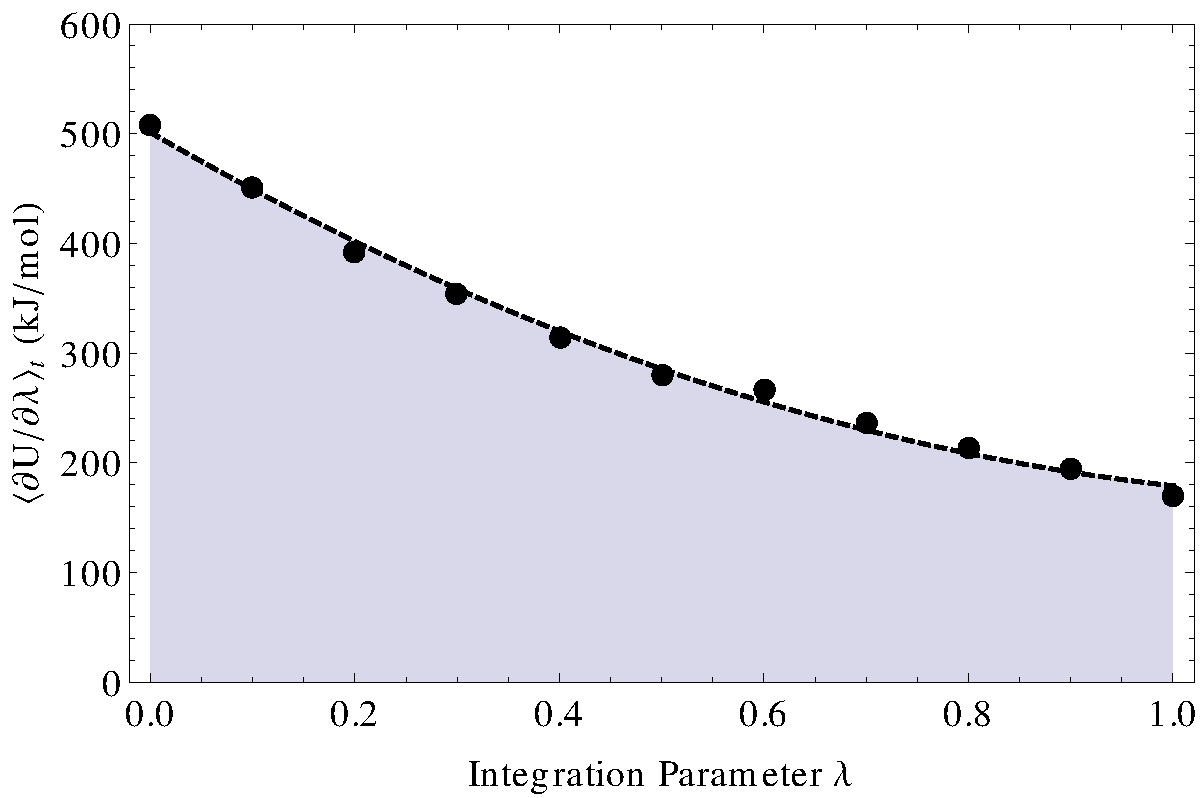
\includegraphics[width=.6\textwidth]{dudl_of_l}
            \end{figure}
        \item The integrate of which is $\Delta G_{\text{transmut},A\rightarrow B\text{ in S}}$, the associated reversible work
    \end{enumerate}
\end{frame}
%~ 
%~ 
%~ 
%~ 
\begin{frame}
    \frametitle{LiF-ThF$_4$}
    %~ donner temp et concentration effect (on a ?) et expliquer le manque de reference
    %~ donc on passe à des objets pour lesquels on a des références 
    Work in progress. Only 600 $^{\circ}$C and 22 mole \% ThF$_4$ for now.
    \vspace{0.5cm}
    \begin{columns}
        \begin{column}{5cm}
            \begin{figure}
                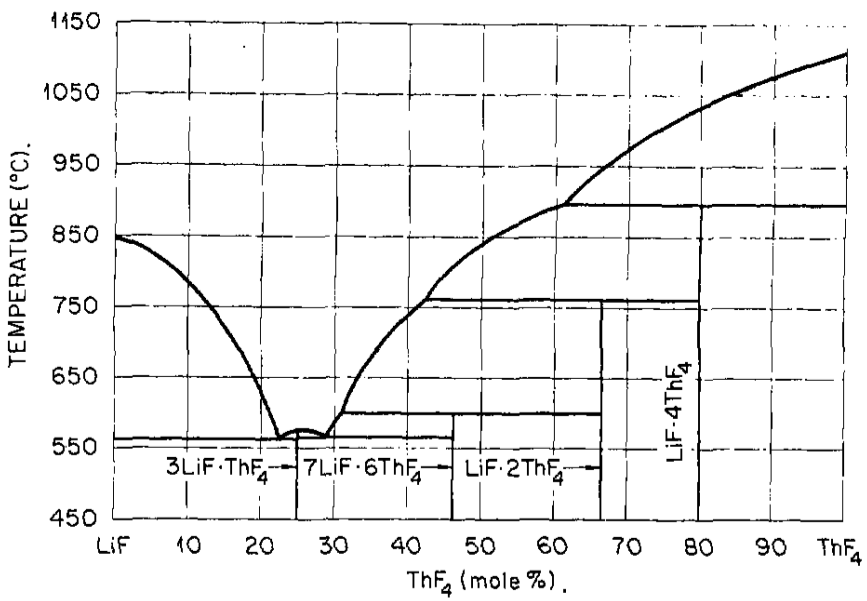
\includegraphics[width=\textwidth]{LiFThF4ddp.png}
            \end{figure}
        \end{column}
        \begin{column}{7cm}
            $\Delta G_{\text{transmut YF}_3 \rightarrow\text{ LaF}_3} = 311.8$ kJ/mol
            \begin{figure}
                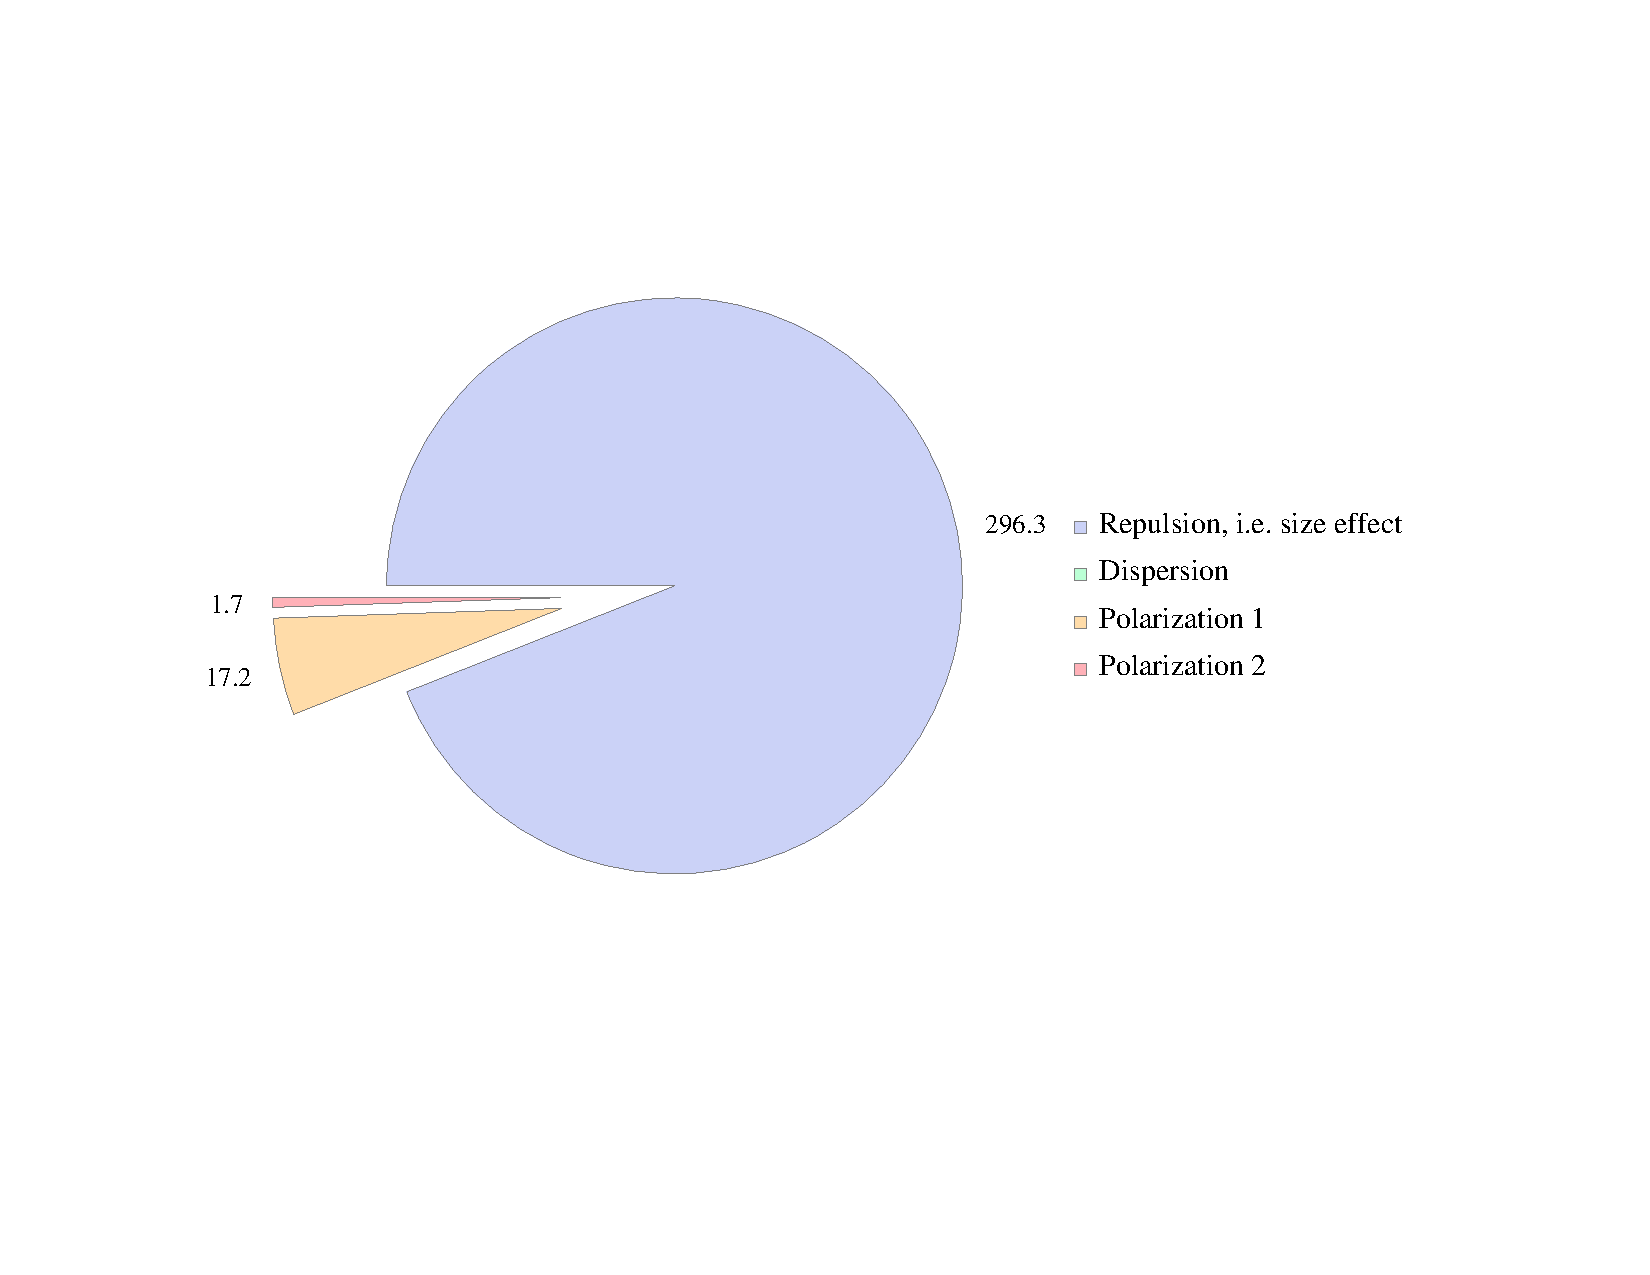
\includegraphics[width=\textwidth]{LiFTF4dGchart}
            \end{figure}
        \end{column}
    \end{columns}
    \begin{itemize}
        \item $\Rightarrow$ Closer look to the "size effect".
    \end{itemize}
\end{frame}
%~ 
%~ 
%~ 
%~ 
\begin{frame}
    \frametitle{Ionic "sizes" as a critical parameter in LiF-ThF$_4$}
    \begin{itemize}
        \item Transmutation of YF$_3$ into LaF$_3$, the "size" of which is decreased from LaF$_3$ to YF$_3$. Polarization etc. unchanged.
        \begin{figure}
            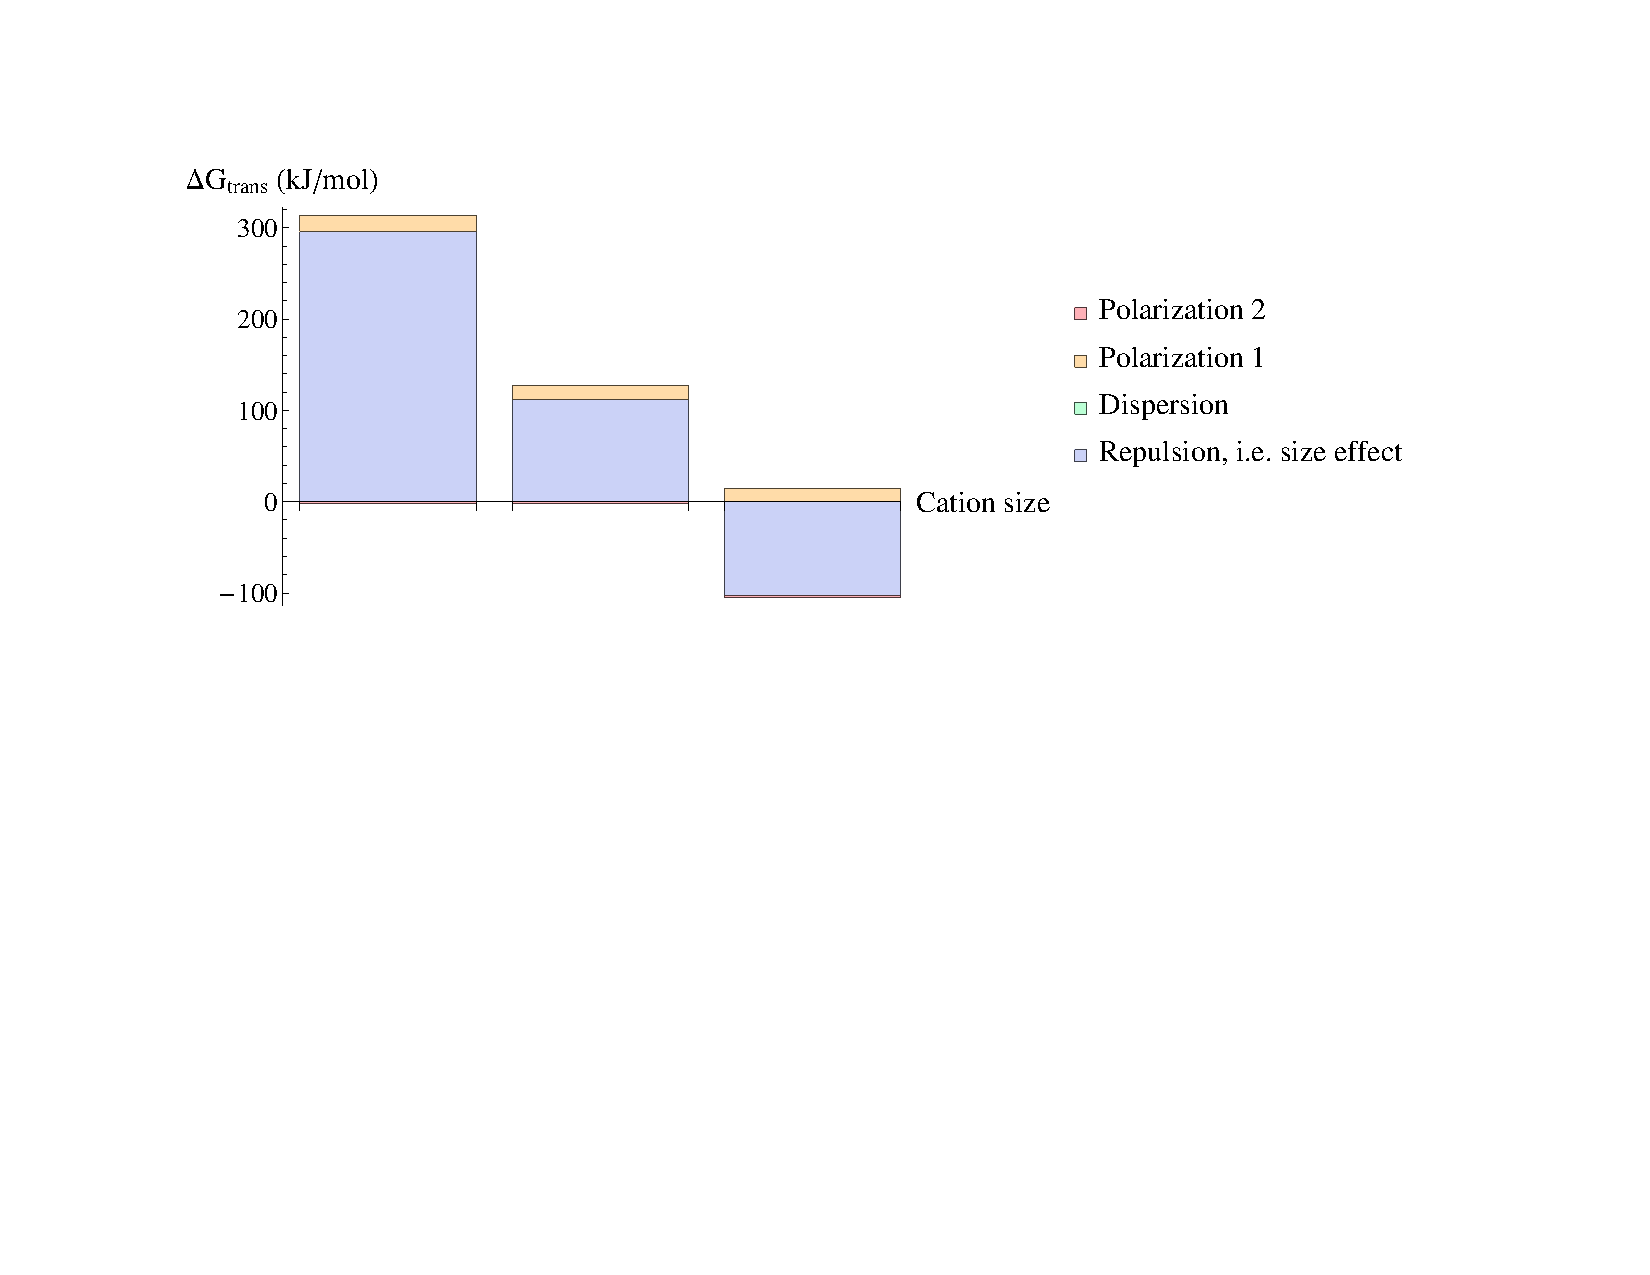
\includegraphics[width=0.9\textwidth]{LiFThF4sizeEffectPiechart}
        \end{figure}
        \item The "size" of the cation drives the free energy of transmutation in LiF-ThF$_4$.
    \end{itemize}
\end{frame}
%~ 
%~ 
%~ 
%~ 
\begin{frame}{Ongoing work on solubilities}{Validation on reference salts NaF-ZrF$_4$ and NaF-BeF$_2$}
    \scriptsize{Ward et al., ORNL report (1959)}
    \begin{columns}
        \begin{column}{6cm}
            \begin{figure}
                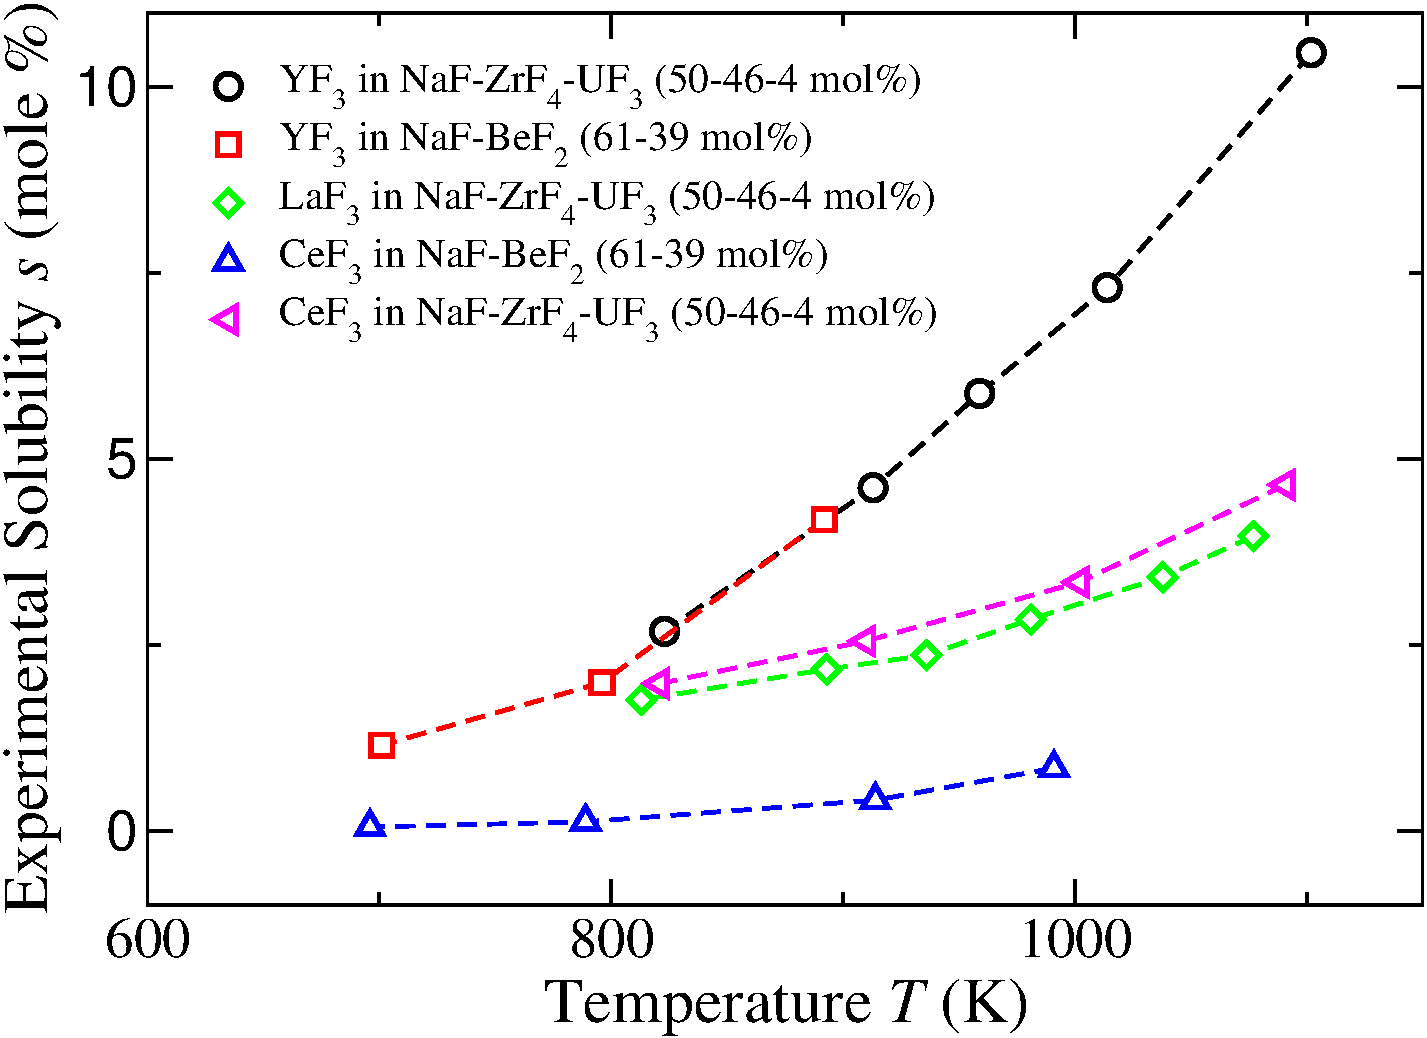
\includegraphics[width=\textwidth]{ward_et_al_solubilities}
            \end{figure}
        \end{column}
        \begin{column}{6cm}
            \begin{figure}
                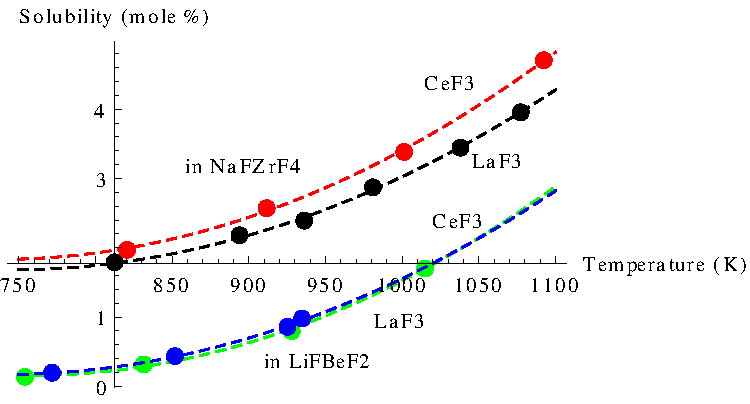
\includegraphics[width=\textwidth]{CeF3vsLaF3}
            \end{figure}
        \end{column}
    \end{columns}
    \begin{itemize}
        \item Solubility of YF$_3$, $s(\text{YF}_3)$, the same in both salts.
        \item Experimentaly, we have $s(\text{YF}_3)$ and $s(\text{LaF}_3)$ or $s(\text{CeF}_3)\approx s(\text{LaF}_3)$ in both salts.
        \item $s(\text{LaF}_3)$ in NaF-ZrF$_4$ $>$ $s(\text{LaF}_3)$ in NaF-BeF$_2$
    \end{itemize}
\end{frame}
%~ 
%~ 
%~ 
%~ 
\begin{frame}{Ongoing work on solubilities}{Validation on reference salts NaF-ZrF$_4$ and NaF-BeF$_2$}
    \begin{figure}
        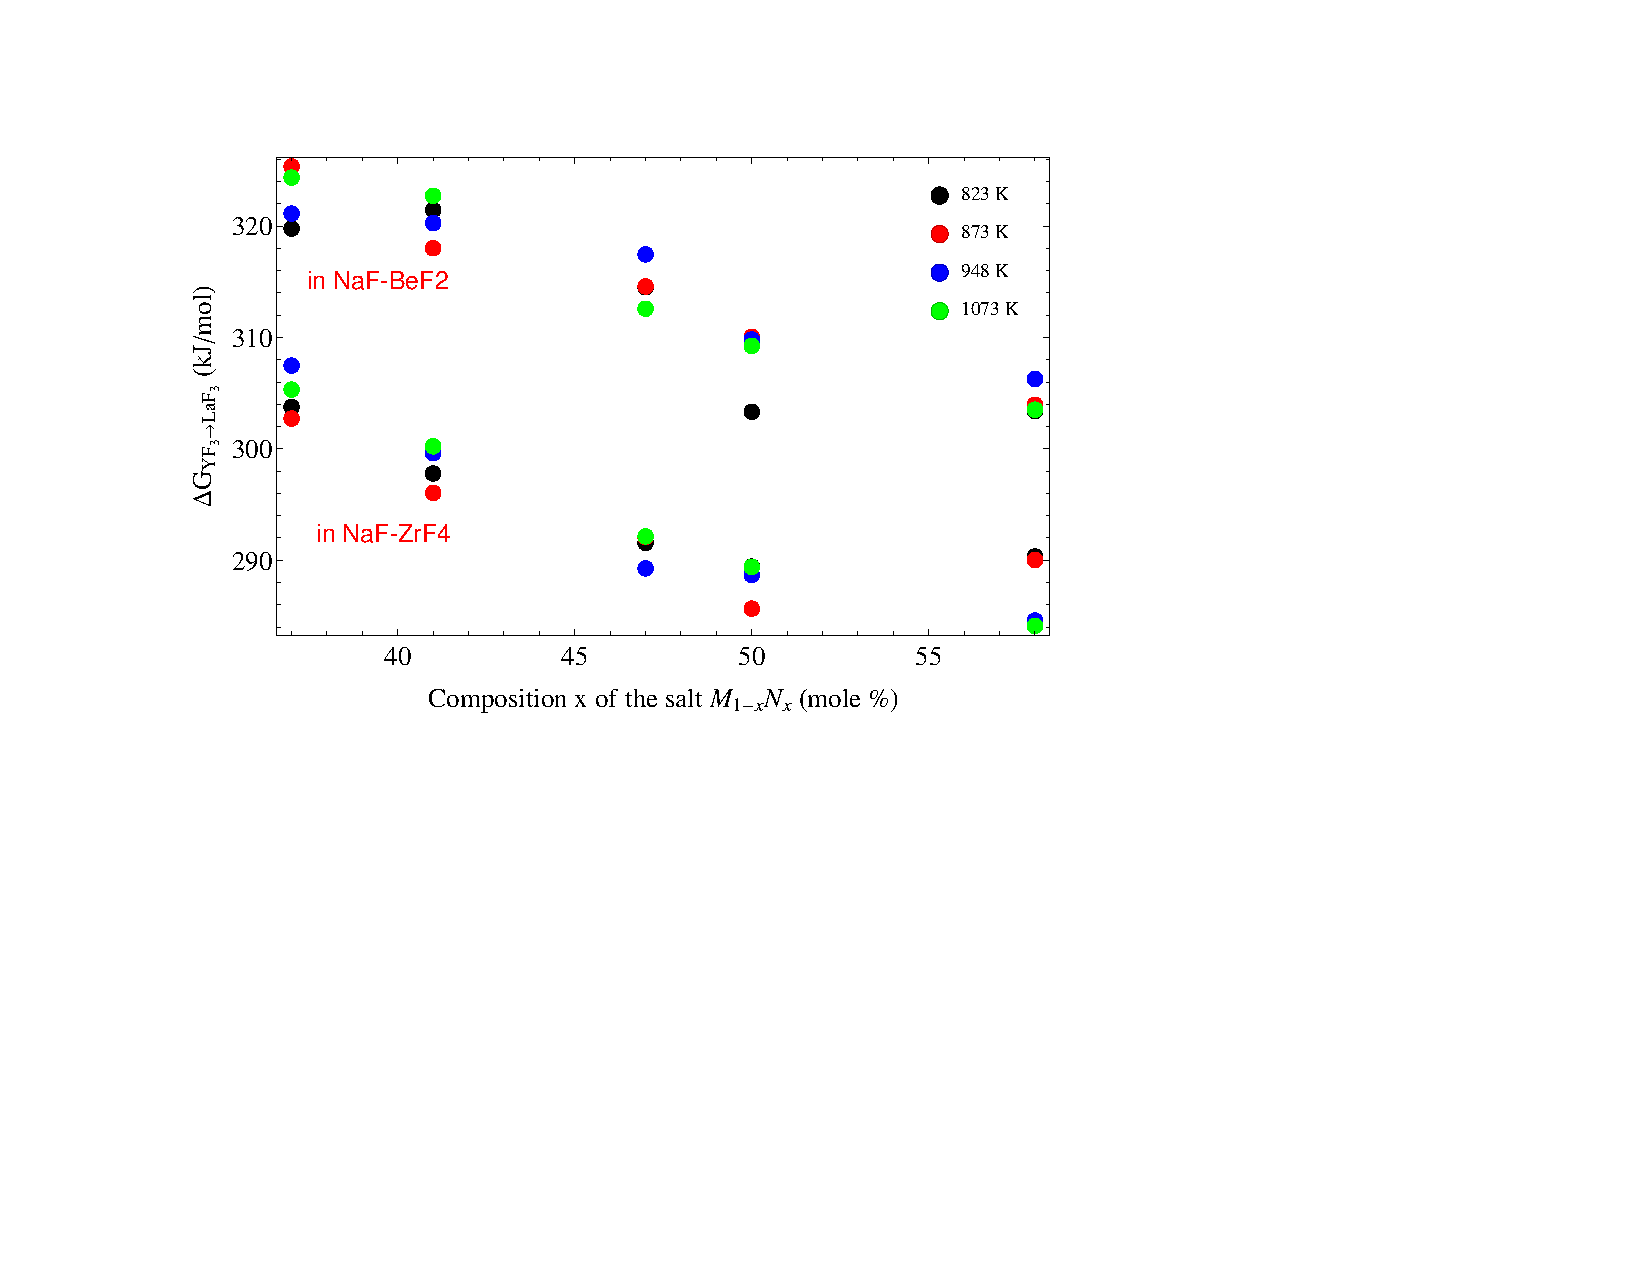
\includegraphics[width=0.6\textwidth]{dGtransZrBe}
    \end{figure}
    \begin{itemize}
        %~ \item $\Delta G_{\text{transmut YF}_3 \rightarrow\text{ LaF}_3$
        \item $\Delta G_{\text{transmut YF}_3 \rightarrow \text{LaF}_3\text{ in NaF-BeF}_2} > \Delta G_{\text{transmut YF}_3 \rightarrow \text{LaF}_3\text{ in NaF-BeF}_2}$
        \item .and. $s(\text{YF}_3)$ the same in both salts
        \item $\Rightarrow$ $s(\text{LaF}_3)$ in NaF-ZrF$_4$ $>$ $s(\text{LaF}_3)$ in NaF-BeF$_2$ \\ Qualitative agreement with exp. Can we be quantitative?
    \end{itemize}
\end{frame}
%~ 
%~ 
%~ 
%~ 
\begin{frame}{Ongoing work on solubilities}{Validation on reference salts NaF-ZrF$_4$ and NaF-BeF$_2$}
    Remember,
    \begin{equation}
        \Delta G_{\text{transmut},A\rightarrow B\text{ in S}} - \Delta G_{\text{transmut},A\rightarrow B\text{ in S}^{\prime}} \approx \beta^{-1}\ln\left(\frac{s_A^S\cdot s_B^{S^\prime}}{s_A^{S^{\prime}}\cdot s_B^S}\right),   \nonumber
    \end{equation}
    .and. $s(\text{YF}_3)$ the same in both salts $\Rightarrow $
    \begin{equation}
        \Delta G_{\text{YF3}\rightarrow\text{LaF3 in NaFZrF4}} - \Delta G_{\text{YF3}\rightarrow\text{LaF3 in NaFBeF2}} \approx \beta^{-1}\ln\left(\frac{s_{\text{LaF}_3}^{\text{NaF-BeF}_2}}{s_{\text{LaF}_3}^{\text{NaF-ZrF}_4}}\right) \nonumber
    \end{equation}
    $\Rightarrow$ Solubility ratio
\end{frame}
%~ 
%~ 
%~ 
%~ 
\begin{frame}{Solubility of LaF$_3$ in NaF-ZrF$_4$ and NaF-BeF$_2$}
    $ r = s_{\text{LaF}_3}^{\text{NaF-BeF}_2} / s_{\text{LaF}_3}^{\text{NaF-ZrF}_4}$
    \begin{columns}
        \begin{column}{6cm}
            \begin{figure}
                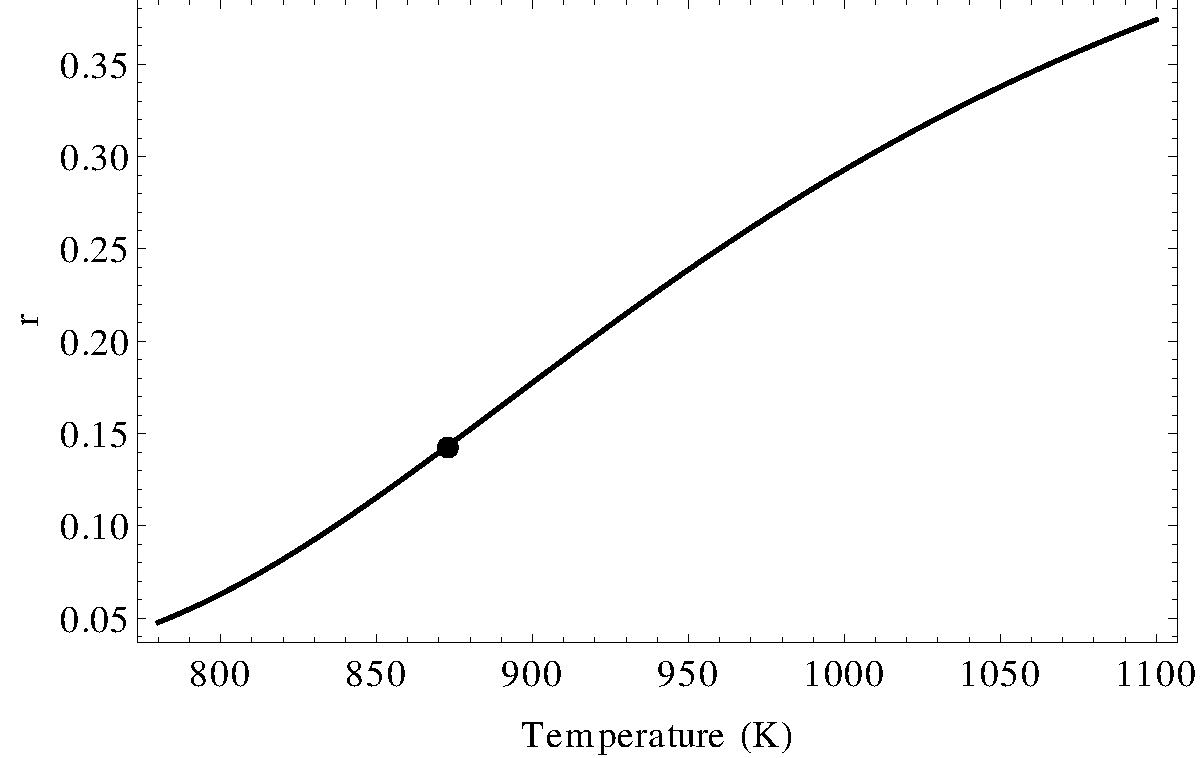
\includegraphics[width=\textwidth]{solRatioEvoWithT}
                \caption{Experimental (Ward et al.): ~~~~~ (NaF)$_{61}$(BeF$_2$)$_{39}$ and (NaF)$_{52}$(ZrF$_4$)$_{48}$}
            \end{figure}
        \end{column}
        \begin{column}{6cm}
            \begin{figure}
                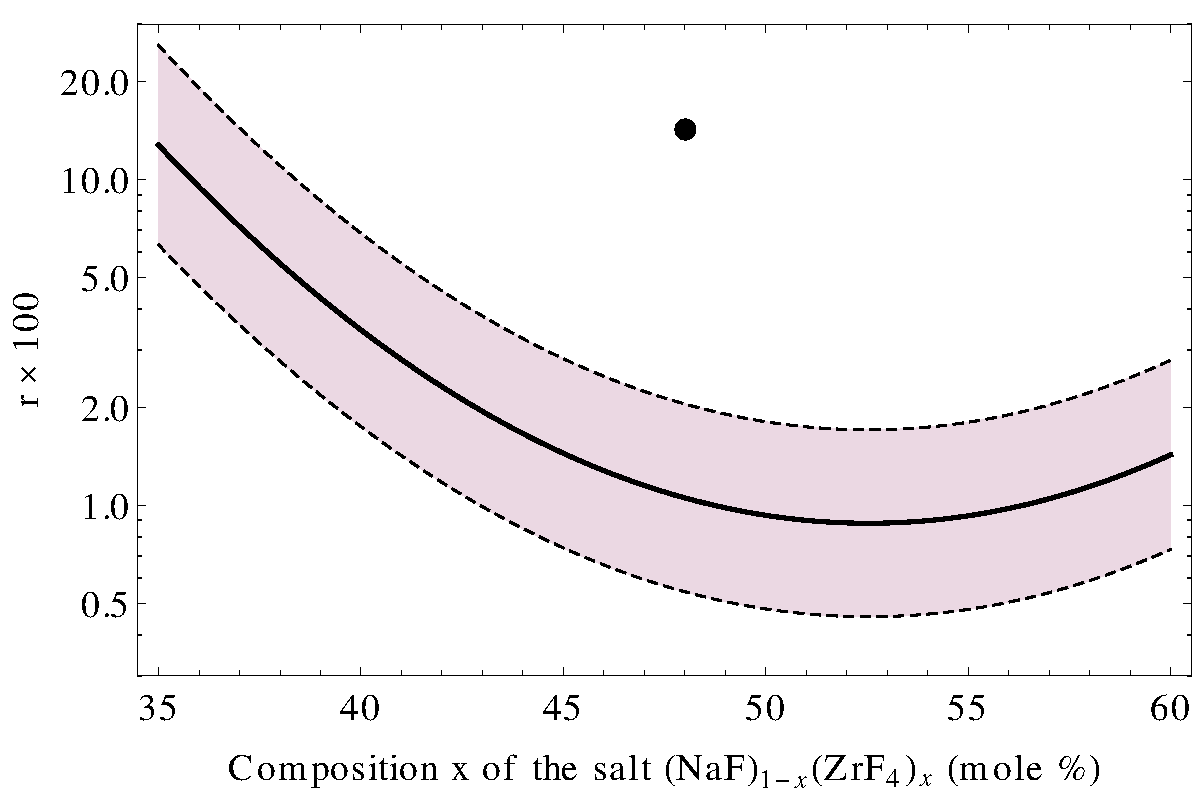
\includegraphics[width=\textwidth]{deducted_solubilities}
                \caption{Calculated: ~~~~~ (NaF)$_{61}$(BeF$_2$)$_{39}$ and 873 K}
            \end{figure}
        \end{column}
    \end{columns}
    Qualitative agreement $\rightarrow$ solubility of LaF$_3$ higher in NaF-ZrF$_4$
    Semi-quantative agreement $r\approx 10^{-1}$
\end{frame}
%~ 
%~ 
%~ 
%~ 
\section{Conclusion \& Perspectives}

\begin{frame}
   \frametitle{Conclusion}
   \begin{itemize}
      \item[$\bullet$] Interaction potentials including many-body polarization effects for a series of molten fluorides
      \item[$\bullet$] Parameterization from first-principles calculations
      \item[$\bullet$] Prediction of transport properties of LiF-ThF$_4$ across the whole range of coompositions/temperatures
      \item[$\bullet$] \alert{Activity coefficients in molten fluorides and relation with solubilities} 
   \end{itemize}
\end{frame}



\begin{frame}{Supplementary material}{Effect of UF$_4$ on solubilities}
    Ward et al. answered in ORNL report (1959)
    \begin{figure}
        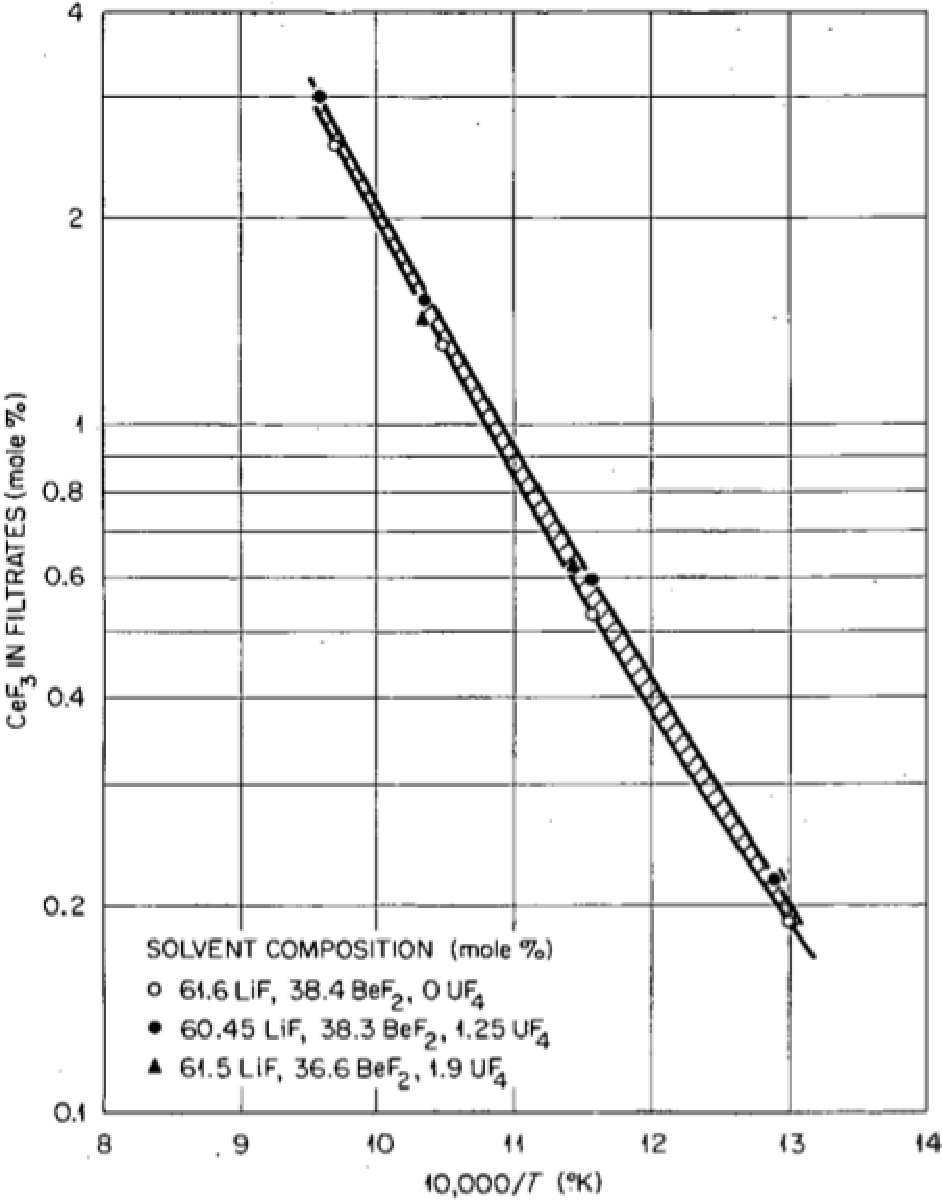
\includegraphics[height=5cm]{UF4effectOnSolubilities}
    \end{figure}
    \begin{itemize}
        \item UF$_4$ has no influence on the solubilities
    \end{itemize}
\end{frame}



\appendix
\makeatletter
  \immediate\write\@mainaux{\string\gdef\string\inserttotalframenumbernew{\insertframenumber}}
\makeatother





\end{document}
